\section{Biểu diễn và Matching Đặc trưng Truyền thống}
\label{sec:feature_representation_and_matching}

\subsection{Dẫn nhập: Từ Đặc trưng Cục bộ đến Biểu diễn Toàn cục}
\label{subsec:local_to_global_representation}

Trong các phần trước, chúng ta đã thành công trong việc trích xuất hàng trăm, thậm chí hàng nghìn, các đặc trưng cục bộ (local features) từ một hình ảnh, ví dụ như các vector SIFT 128 chiều. Mỗi vector này là một "dấu vân tay" số học chi tiết cho một vùng ảnh nhỏ. Tuy nhiên, điều này đặt ra một vấn đề mới và cũng là một thách thức cốt lõi: làm thế nào để tổng hợp (aggregate) tập hợp các đặc trưng có số lượng thay đổi này thành một \textbf{biểu diễn toàn cục (global representation)} duy nhất, có chiều dài cố định cho toàn bộ hình ảnh?

Một biểu diễn toàn cục, có chiều dài cố định là điều kiện tiên quyết cho hầu hết các thuật toán học máy tiêu chuẩn, chẳng hạn như Support Vector Machines (SVM) hay các bộ phân loại tuyến tính khác, vốn yêu cầu một vector đầu vào có kích thước nhất quán. Chúng ta không thể đưa trực tiếp một "túi" chứa 500 vector SIFT cho ảnh này và 800 vector SIFT cho ảnh khác vào một bộ phân loại.

Nhiệm vụ của chương này là khám phá các phương pháp kinh điển được thiết kế để giải quyết chính xác bài toán này: xây dựng một cây cầu nối từ thế giới của các đặc trưng cục bộ, rời rạc sang một không gian vector toàn cục, có cấu trúc. Các phương pháp này, dù ra đời trước kỷ nguyên học sâu, lại ẩn chứa những ý tưởng nền tảng sâu sắc về lượng tử hóa, mã hóa, và thống kê, những ý tưởng vẫn còn nguyên giá trị cho đến ngày nay. Chúng ta sẽ bắt đầu với phương pháp có sức ảnh hưởng và dễ hiểu nhất: Bag of Visual Words.

\subsection{Bag of Visual Words (BoVW): Từ vựng cho Hình ảnh}
\label{subsec:bovw}

Mô hình \textbf{Bag of Visual Words (BoVW)}, hay còn gọi là Bag of Features, được lấy cảm hứng trực tiếp từ một kỹ thuật rất thành công trong lĩnh vực xử lý ngôn ngữ tự nhiên (NLP) và truy xuất thông tin (Information Retrieval) gọi là "Bag of Words".

\begin{mdframed}[style=infobox]
    \textbf{Trực giác: Phép tương đồng giữa Văn bản và Hình ảnh}
    
    Hãy tưởng tượng cách chúng ta phân loại các tài liệu văn bản. Một cách tiếp cận đơn giản nhưng hiệu quả là bỏ qua hoàn toàn ngữ pháp và thứ tự từ, chỉ cần đếm tần suất xuất hiện của mỗi từ trong một cuốn từ điển chung. Một tài liệu về "vật lý thiên văn" sẽ chứa nhiều từ như "sao", "thiên hà", "lỗ đen", trong khi một tài liệu về "sinh học" sẽ có nhiều từ "tế bào", "gen", "ADN". Histogram tần suất từ này trở thành một vector đặc trưng cho tài liệu đó.
    
    Mô hình BoVW áp dụng chính xác phép tương đồng này cho hình ảnh:
    \begin{itemize}
        \item \textbf{Tài liệu (Document)} $\rightarrow$ \textbf{Hình ảnh (Image)}
        \item \textbf{Từ (Word)} $\rightarrow$ \textbf{Đặc trưng cục bộ (ví dụ: vector SIFT)}
        \item \textbf{Từ điển (Dictionary)} $\rightarrow$ \textbf{Sổ mã/Từ điển Thị giác (Codebook/Visual Vocabulary)}
        \item \textbf{Histogram tần suất từ} $\rightarrow$ \textbf{Histogram tần suất "Từ Thị giác"}
    \end{itemize}
    Ý tưởng cốt lõi là biểu diễn một hình ảnh bằng một histogram cho biết "từ thị giác" nào xuất hiện và với tần suất bao nhiêu, bỏ qua hoàn toàn thông tin về vị trí không gian của chúng.
\end{mdframed}

Quy trình xây dựng và sử dụng mô hình BoVW bao gồm hai giai đoạn chính: (1) Giai đoạn offline để học từ điển, và (2) Giai đoạn online để biểu diễn một ảnh mới. Quy trình này thường được chia thành các bước sau:

\subsubsection{Bước 1: Trích xuất Đặc trưng Cục bộ (Local Feature Extraction)}
\label{subsubsec:bovw_extraction}
Đây là bước khởi đầu, đóng vai trò nền tảng cho toàn bộ quy trình. Đối với một tập hợp lớn các hình ảnh huấn luyện (training images), chúng ta áp dụng các thuật toán đã học ở phần trước như SIFT, SURF, hoặc ORB để trích xuất các đặc trưng cục bộ.
\begin{itemize}
    \item \textbf{Mục tiêu:} Thu thập một tập hợp đa dạng và phong phú các vector đặc trưng, đại diện cho nhiều loại cấu trúc hình ảnh (góc, cạnh, đốm màu, kết cấu,...) có thể xuất hiện trong bộ dữ liệu.
    \item \textbf{Kết quả:} Một tập hợp khổng lồ $\mathcal{X}_{train} = \{\mathbf{x}_1, \mathbf{x}_2, ..., \mathbf{x}_M\}$ gồm $M$ vector đặc trưng. Ví dụ, từ 10,000 ảnh huấn luyện, mỗi ảnh có trung bình 500 đặc trưng SIFT, chúng ta sẽ có $M = 5,000,000$ vector SIFT 128 chiều. Tập hợp này là nguyên liệu thô để xây dựng từ điển.
\end{itemize}

\subsubsection{Bước 2: Học Từ điển Thị giác (Visual Vocabulary Generation)}
\label{subsubsec:bovw_codebook}
\textbf{Mục tiêu:} Xây dựng một "từ điển" gồm $K$ "từ thị giác" (visual words) đại diện. Không gian của các vector SIFT là không gian vector liên tục. Để tạo ra một từ điển hữu hạn, chúng ta cần phải lượng tử hóa (quantize) không gian này. Phương pháp phổ biến nhất để làm điều này là sử dụng thuật toán phân cụm \textbf{k-means}.

\begin{enumerate}
    \item \textbf{Đầu vào:} Toàn bộ tập hợp các vector đặc trưng cục bộ $\mathcal{X}_{train}$ đã được trích xuất.
    \item \textbf{Thuật toán:} Thuật toán k-means được áp dụng trên tập hợp vector này để tìm ra $K$ tâm cụm (centroids). Mục tiêu của k-means là tìm ra một tập hợp các tâm cụm $\mathcal{V} = \{\mathbf{v}_1, ..., \mathbf{v}_K\}$ và một phân hoạch của $\mathcal{X}_{train}$ thành $K$ cụm $C_1, ..., C_K$ sao cho tổng bình phương khoảng cách từ mỗi điểm dữ liệu đến tâm cụm gần nhất của nó được tối thiểu hóa. Công thức toán học của hàm mục tiêu (objective function) được biểu diễn như sau (tương đương với công thức (2) trong \cite{Gidaris2020}):
    \begin{equation}
        \underset{\mathcal{V}}{\operatorname{min}} \sum_{\mathbf{x} \in \mathcal{X}_{train}} \min_{k=1,...,K} ||\mathbf{x} - \mathbf{v}_k||_2^2
        \label{eq:kmeans_objective}
    \end{equation}
    Trong đó:
    \begin{itemize}
        \item $\mathbf{x}$ là một vector đặc trưng cục bộ trong tập huấn luyện.
        \item $\mathbf{v}_k$ là vector tâm của cụm thứ $k$.
        \item $||\cdot||_2^2$ là bình phương khoảng cách Euclid.
    \end{itemize}
    \item \textbf{Đầu ra:} Tập hợp $K$ tâm cụm $\mathcal{V} = \{\mathbf{v}_1, \mathbf{v}_2, ..., \mathbf{v}_K\}$. Mỗi tâm cụm $\mathbf{v}_k$, vốn cũng là một vector D-chiều (ví dụ 128-D cho SIFT), chính là một \textbf{"từ thị giác" (visual word)}. Toàn bộ tập hợp $\mathcal{V}$ này tạo thành \textbf{sổ mã (codebook)} hay \textbf{từ điển thị giác}.
\end{enumerate}

\begin{center}
    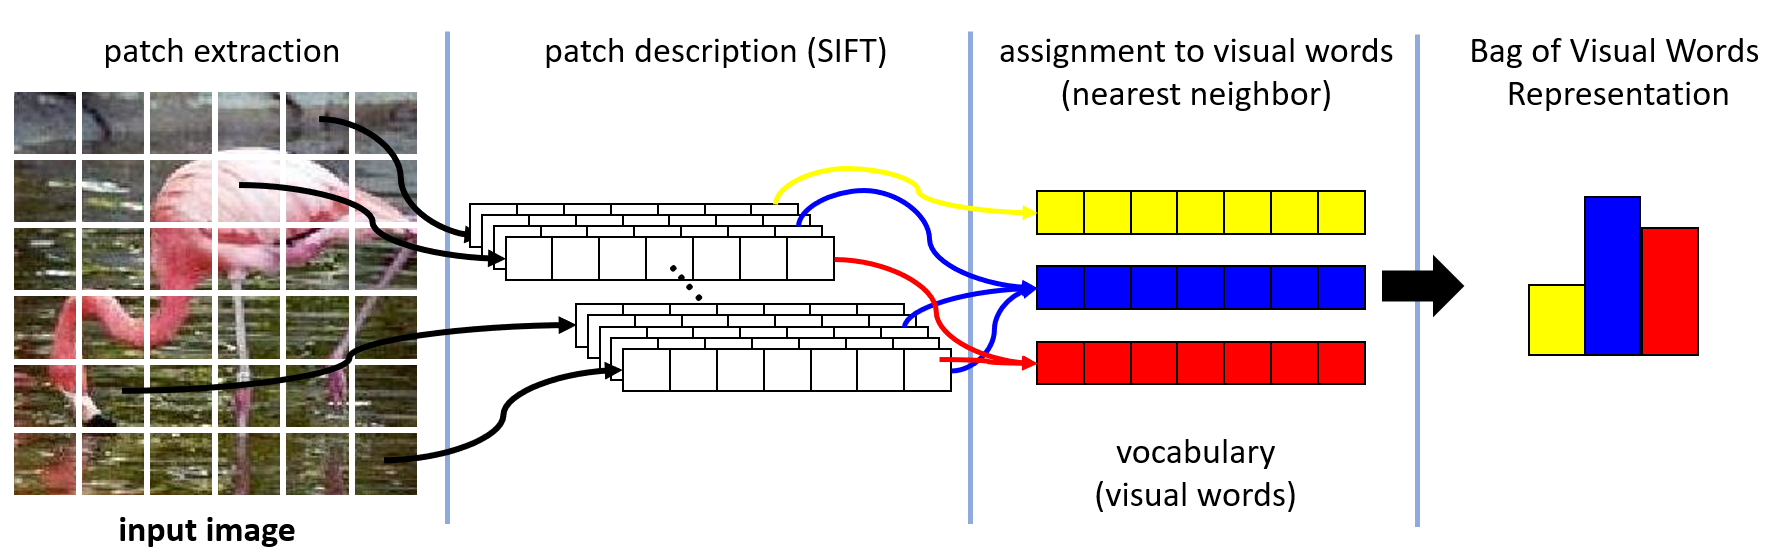
\includegraphics[width=1.0\textwidth]{images/visual_word_cluster_members.png}
    \captionof{figure}{Minh họa các "từ thị giác". Mỗi hàng là các vùng ảnh gần nhất với một tâm cụm (từ thị giác). Có thể thấy các từ thị giác mã hóa các cấu trúc lặp lại như mắt, bánh xe, hoặc các mảng kết cấu.}
    \label{fig:visual_word_clusters}
\end{center}

Kích thước của từ điển, $K$, là một siêu tham số (hyperparameter) cực kỳ quan trọng. Việc lựa chọn $K$ là một sự đánh đổi:
\begin{itemize}
    \item \textbf{K nhỏ (ví dụ: 100-500):} Từ vựng sẽ rất thô. Nhiều vùng ảnh có cấu trúc khác biệt có thể bị gộp vào cùng một "từ thị giác", làm giảm khả năng phân biệt của mô hình.
    \item \textbf{K lớn (ví dụ: 10,000-1,000,000):} Từ vựng sẽ chi tiết và có tính phân biệt cao hơn. Tuy nhiên, nó đòi hỏi chi phí tính toán lớn hơn đáng kể cho việc phân cụm và xây dựng histogram. Ngoài ra, histogram kết quả có thể trở nên rất thưa thớt (sparse), gây khó khăn cho các bộ phân loại.
\end{itemize}

\subsubsection{Bước 3: Lượng tử hóa và Biểu diễn Ảnh (Image Representation via Quantization)}
\label{subsubsec:bovw_quantization}
Sau khi đã có từ điển $\mathcal{V}$, chúng ta có thể biểu diễn bất kỳ hình ảnh mới nào (dù có trong tập huấn luyện hay không) bằng một vector BoVW.

\begin{enumerate}
    \item \textbf{Trích xuất Đặc trưng:} Trích xuất tất cả $N$ vector đặc trưng cục bộ $\{\mathbf{x}_1, ..., \mathbf{x}_N\}$ từ ảnh mới.
    
    \item \textbf{Lượng tử hóa Vector (Vector Quantization - VQ):} Đối với mỗi vector đặc trưng $\mathbf{x}_i$ của ảnh, chúng ta tìm "từ thị giác" $\mathbf{v}_k$ gần nhất với nó trong từ điển. Quá trình này gán cho mỗi $\mathbf{x}_i$ một chỉ số $q_i \in \{1, ..., K\}$.
    \begin{equation}
        q_i = \underset{k \in \{1, ..., K\}}{\operatorname{argmin}} ||\mathbf{x}_i - \mathbf{v}_k||_2^2
        \label{eq:bovw_assignment}
    \end{equation}
    Đây được gọi là \textbf{gán cứng (hard assignment)}, vì mỗi đặc trưng được gán cho chính xác một từ thị giác, bỏ qua khoảng cách thực tế hay khả năng nó có thể thuộc về các từ khác.
    
    \item \textbf{Tổng hợp (Aggregation) thành Histogram:} Dựa trên tập hợp các chỉ số $\{q_1, ..., q_N\}$, chúng ta xây dựng một vector histogram $\mathbf{h} \in \mathbb{R}^K$. Có hai cách phổ biến để tổng hợp, như được đề cập trong \cite{Gidaris2020}:
    \begin{description}
        \item[Histogram BoVW (Đếm tần suất):] Mỗi thành phần $h_k$ của histogram đếm số lần từ thị giác thứ $k$ xuất hiện trong ảnh.
        \begin{equation}
            h_k = \sum_{i=1}^{N} \mathbb{I}[q_i = k]
            \label{eq:bovw_histogram_count}
        \end{equation}
        trong đó $\mathbb{I}[\cdot]$ là hàm chỉ thị (indicator function), trả về 1 nếu điều kiện bên trong là đúng, và 0 nếu ngược lại.
        \item[Binary BoVW (Đếm sự hiện diện):] Mỗi thành phần $h_k$ chỉ đơn giản cho biết liệu từ thị giác thứ $k$ có xuất hiện trong ảnh ít nhất một lần hay không.
        \begin{equation}
            h_k = \max_{i=1,...,N} \mathbb{I}[q_i = k]
            \label{eq:bovw_binary_count}
        \end{equation}
        Vector kết quả sẽ là một vector nhị phân. Phương pháp này hữu ích khi sự bùng nổ của một loại đặc trưng nào đó (burstiness) có thể làm sai lệch histogram tần suất.
    \end{description}
    
    \item \textbf{Chuẩn hóa (Normalization):} Để biểu diễn không phụ thuộc vào số lượng đặc trưng trong ảnh, histogram $\mathbf{h}$ thường được chuẩn hóa. Các phương pháp phổ biến bao gồm:
    \begin{itemize}
        \item \textbf{Chuẩn hóa L1:} $\mathbf{h}_{norm} = \mathbf{h} / ||\mathbf{h}||_1 = \mathbf{h} / \sum_k |h_k|$. Vector kết quả có thể được xem như một phân bố xác suất.
        \item \textbf{Chuẩn hóa L2:} $\mathbf{h}_{norm} = \mathbf{h} / ||\mathbf{h}||_2 = \mathbf{h} / \sqrt{\sum_k h_k^2}$. Vector kết quả nằm trên một siêu cầu đơn vị, là lựa chọn phổ biến khi sử dụng với các kernel tuyến tính (ví dụ trong SVM).
    \end{itemize}
\end{enumerate}
Vector $\mathbf{h}_{norm}$ chính là biểu diễn BoVW cuối cùng của hình ảnh, sẵn sàng để được đưa vào các thuật toán phân loại.

\begin{center}
    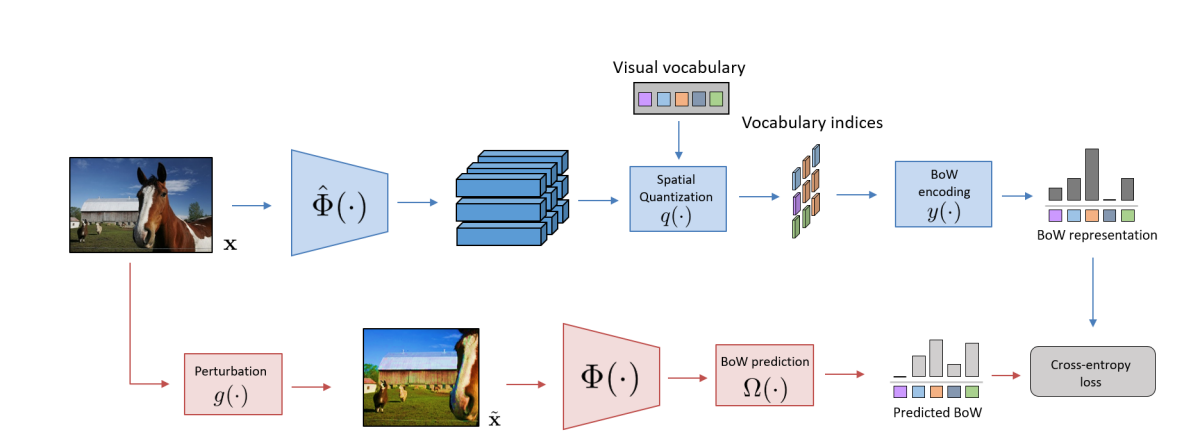
\includegraphics[width=1.0\textwidth]{images/bovw_pipeline.png}
    \captionof{figure}{Quy trình Bag of Visual Words cổ điển. (1) Trích xuất các đặc trưng cục bộ (ví dụ: SIFT) từ một tập ảnh huấn luyện. (2) Phân cụm tất cả các đặc trưng này bằng k-means để tạo ra một từ điển thị giác gồm K "từ thị giác". (3) Đối với một ảnh mới, trích xuất đặc trưng và gán mỗi đặc trưng cho từ thị giác gần nhất trong từ điển (lượng tử hóa). (4) Xây dựng một histogram tần suất K chiều bằng cách đếm số lần xuất hiện của mỗi từ thị giác. Vector này, sau khi chuẩn hóa, là biểu diễn cuối cùng của ảnh.}
    \label{fig:bovw_pipeline}
\end{center}

\subsubsection{BoVW trong Kỷ nguyên Học sâu: Một Góc nhìn Hiện đại}
\label{subsubsec:bovw_deep_learning}
Mô hình BoVW cổ điển sử dụng các đặc trưng thủ công như SIFT. Tuy nhiên, ý tưởng cốt lõi của BoVW — lượng tử hóa không gian đặc trưng và tổng hợp thành histogram — vẫn còn rất mạnh mẽ. Trong bối cảnh hiện đại, BoVW đã được tái sinh theo hai cách chính:

\begin{enumerate}
    \item \textbf{Sử dụng Đặc trưng Sâu (Deep Features):} Thay vì SIFT, chúng ta có thể sử dụng các Mạng nơ-ron Tích chập (CNN) đã được huấn luyện trước (pre-trained) để trích xuất các đặc trưng. Các feature map từ các lớp sâu của CNN (ví dụ: lớp tích chập cuối cùng của ResNet) được coi là một tập hợp các đặc trưng cục bộ dày đặc. Quá trình học từ điển k-means và xây dựng histogram sau đó được thực hiện trên các "đặc trưng sâu" này.
    
    \item \textbf{BoVW như một Tác vụ Tự giám sát (Self-Supervised Pretext Task):} Đây chính là ý tưởng đột phá trong paper của Gidaris et al. \cite{Gidaris2020}. Thay vì chỉ là một phương pháp biểu diễn, BoVW có thể trở thành mục tiêu để một mạng nơ-ron học. Quy trình này như sau:
    \begin{itemize}
        \item \textbf{Giai đoạn 1 (Tạo "Ground Truth" BoVW):}
            \begin{enumerate}
                \item Huấn luyện một mạng nơ-ron cơ sở (base convnet) $\Phi_{base}$ bằng một tác vụ tự giám sát đơn giản (ví dụ: dự đoán góc xoay của ảnh).
                \item Sử dụng $\Phi_{base}$ để trích xuất các feature map từ tất cả các ảnh trong bộ dữ liệu không nhãn.
                \item Thực hiện k-means trên các vector đặc trưng này để tạo ra một từ điển thị giác $\mathcal{V}$.
                \item Đối với mỗi ảnh gốc $I_{orig}$ trong bộ dữ liệu, tính toán vector BoVW của nó, $y(I_{orig})$, và coi đây là "nhãn" ground truth.
            \end{enumerate}
        \item \textbf{Giai đoạn 2 (Học biểu diễn bằng cách dự đoán BoVW):}
            \begin{enumerate}
                \item Lấy một mạng nơ-ron mới, $\Phi_{new}$, khởi tạo ngẫu nhiên.
                \item Nhiệm vụ của $\Phi_{new}$ là: nhận đầu vào là một phiên bản bị biến dạng (perturbed) của ảnh gốc, $I_{pert} = g(I_{orig})$ (ví dụ: bị cắt cúp, thay đổi màu sắc), và phải dự đoán vector BoVW của ảnh gốc, $y(I_{orig})$.
                \item Mạng được huấn luyện để tối thiểu hóa sai khác giữa BoVW dự đoán và BoVW ground truth, thường sử dụng hàm mất mát cross-entropy:
                \begin{equation}
                    \mathcal{L} = \mathbb{E}_{I \sim \mathcal{D}} \left[ \text{CrossEntropy}(\Omega(\Phi_{new}(g(I))), y(I)) \right]
                    \label{eq:bovw_ssl_loss}
                \end{equation}
                Trong đó $\Omega$ là một lớp tuyến tính (prediction head) để ánh xạ từ biểu diễn của $\Phi_{new}$ ra phân bố xác suất trên các từ thị giác.
            \end{enumerate}
    \end{itemize}
    \textbf{Trực giác của phương pháp này:} Để có thể dự đoán BoVW của ảnh gốc từ một mảnh cắt cúp, mạng $\Phi_{new}$ buộc phải học các biểu diễn có ý nghĩa ngữ nghĩa, có khả năng suy luận về bối cảnh (context) và bất biến với các phép biến dạng. Đây là một tín hiệu học tập mạnh mẽ hơn nhiều so với việc chỉ tái tạo lại pixel.
\end{enumerate}

\subsubsection{Hạn chế và Cải tiến}
Mô hình BoVW, dù ở dạng cổ điển hay hiện đại, vẫn có những nhược điểm cố hữu.
\begin{description}
    \item[Mất thông tin Lượng tử hóa:] "Gán cứng" là một nguồn mất mát thông tin lớn. Một đặc trưng có thể nằm chính xác giữa hai từ thị giác, nhưng bị buộc phải chọn một, bỏ qua sự không chắc chắn này. Các phương pháp "gán mềm" (soft assignment) đã được đề xuất để khắc phục, nhưng chúng ta sẽ thảo luận kỹ hơn về chúng trong các phần sau về Fisher Vector và VLAD.
    \item[Mất thông tin Không gian:] Nhược điểm lớn nhất của BoVW là nó hoàn toàn bỏ qua vị trí và mối quan hệ không gian giữa các đặc trưng. Một ảnh chứa mặt người và một ảnh khác có các đặc trưng tương tự nhưng bị xáo trộn vị trí ngẫu nhiên sẽ có cùng biểu diễn BoVW.
\begin{center}
    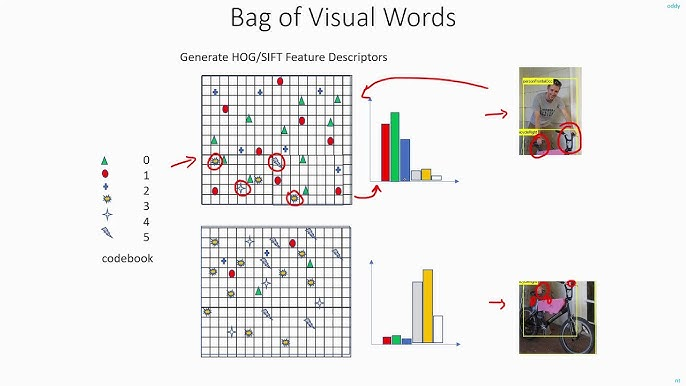
\includegraphics[width=0.8\textwidth]{images/bovw_spatial_limitation.jpg}
    \captionof{figure}{Hạn chế của BoVW: Cả hai ảnh (trên và dưới) đều chứa các "từ thị giác" tương tự (mắt, mũi, miệng) và do đó có thể tạo ra histogram BoVW gần giống nhau, dù cấu trúc không gian hoàn toàn khác biệt.}
    \label{fig:bovw_spatial_limitation}
\end{center}
        \begin{itemize}
            \item \textbf{Giải pháp - Spatial Pyramid Matching (SPM):} Một cải tiến kinh điển là SPM \cite{Lazebnik2006}. Thay vì tính một histogram toàn cục, ảnh được chia thành một lưới các vùng (ví dụ $2 \times 2$), và một histogram BoVW được tính cho mỗi vùng. Các histogram này sau đó được nối lại. Quá trình này được lặp lại ở các độ phân giải lưới khác nhau (ví dụ $1 \times 1, 2 \times 2, 4 \times 4$) để tạo ra một biểu diễn giữ lại thông tin không gian ở nhiều cấp độ.
        \end{itemize}
\begin{center}
    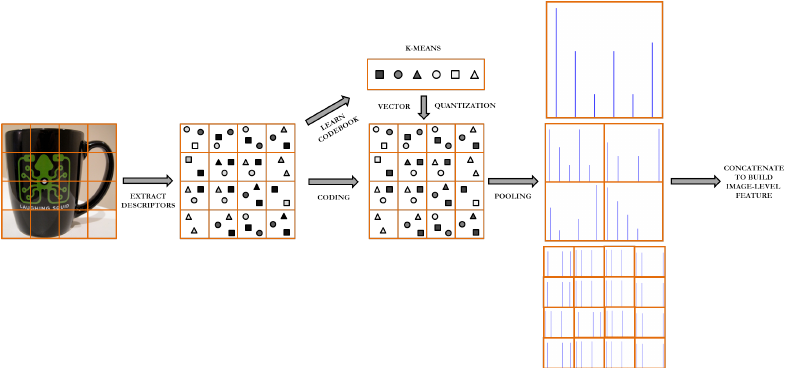
\includegraphics[width=0.9\textwidth]{images/spatial_pyramid_matching.png}
    \captionof{figure}{Minh họa Spatial Pyramid Matching (SPM). Ảnh được chia thành các lưới ở nhiều cấp độ (1x1, 2x2, 4x4). Một histogram BoVW được tính trên mỗi vùng và tất cả được nối lại, giúp giữ lại thông tin không gian.}
    \label{fig:spatial_pyramid_matching}
\end{center}
    \item[Semantic Gap:] Các từ thị giác được tạo ra bởi k-means dựa trên sự tương đồng về mặt hình học trong không gian đặc trưng, không nhất thiết phải tương ứng với các khái niệm ngữ nghĩa mà con người hiểu. Mặc dù hình minh họa cho thấy sự tương quan, nhưng điều này không phải lúc nào cũng đúng.
\end{description}

Những hạn chế này, đặc biệt là về việc mất thông tin lượng tử hóa, chính là động lực cho sự ra đời của các phương pháp kế nhiệm tinh vi hơn như Fisher Vector và VLAD, mà chúng ta sẽ khám phá ngay sau đây.

\subsection{Fisher Vectors (FV): Vượt ra ngoài Việc đếm}
\label{subsec:fisher_vectors}

Nếu BoVW là việc "đếm" các từ thị giác, thì \textbf{Fisher Vector (FV)} \cite{Sanchez2013} là một bước tiến vượt bậc bằng cách mô tả một cách chi tiết hơn sự phân bố của các đặc trưng trong ảnh. Thay vì chỉ hỏi \textit{"Từ thị giác nào xuất hiện?"}, FV hỏi một câu hỏi tinh vi hơn: \textit{"Tập hợp các đặc trưng trong ảnh này khác biệt như thế nào so với một mô hình phân bố chung của tất cả các đặc trưng thị giác?"}.

FV được xây dựng dựa trên một khái niệm lý thuyết từ thống kê gọi là \textbf{Fisher Kernel} \cite{Jaakkola1999}. Ý tưởng cốt lõi là biểu diễn một mẫu dữ liệu (ở đây là một hình ảnh) bằng vector gradient của hàm log-likelihood của mẫu đó đối với các tham số của một mô hình xác suất sinh (generative probability model). Vector gradient này, được gọi là \textbf{Fisher score}, mô tả hướng trong không gian tham số mà các tham số của mô hình cần được điều chỉnh để phù hợp nhất với dữ liệu quan sát được.

\subsubsection{Nền tảng lý thuyết: Từ Fisher Kernel đến Fisher Vector}
\label{subsubsec:fv_theory}
Let $p(\mathbf{x}|\boldsymbol{\lambda})$ là một hàm mật độ xác suất (probability density function - pdf) mô tả quá trình sinh ra các đặc trưng $\mathbf{x}$, với $\boldsymbol{\lambda}$ là vector chứa $M$ tham số của mô hình. Cho một tập hợp $N$ quan sát $\mathbf{X} = \{\mathbf{x}_1, ..., \mathbf{x}_N\}$, \textbf{Fisher score} của $\mathbf{X}$ được định nghĩa là:
\begin{equation}
    \mathcal{G}_{\boldsymbol{\lambda}}^{\mathbf{X}} = \nabla_{\boldsymbol{\lambda}} \log p(\mathbf{X}|\boldsymbol{\lambda})
    \label{eq:fisher_score}
\end{equation}
Vector này có chiều $M \times 1$. Nó cho biết mỗi tham số của mô hình đã đóng góp như thế nào vào quá trình sinh ra tập dữ liệu $\mathbf{X}$.

Tuy nhiên, không gian của các Fisher score không phải là không gian Euclid thông thường. Để định nghĩa một tích vô hướng hợp lệ trong không gian này, Jaakkola và Haussler đã đề xuất \textbf{Fisher Kernel}, một kernel đo lường sự tương đồng giữa hai tập quan sát $\mathbf{X}$ và $\mathbf{Y}$:
\begin{equation}
    K_{FK}(\mathbf{X}, \mathbf{Y}) = (\mathcal{G}_{\boldsymbol{\lambda}}^{\mathbf{X}})^T \mathbf{F}_{\boldsymbol{\lambda}}^{-1} \mathcal{G}_{\boldsymbol{\lambda}}^{\mathbf{Y}}
    \label{eq:fisher_kernel}
\end{equation}
trong đó $\mathbf{F}_{\boldsymbol{\lambda}}$ là \textbf{Ma trận Thông tin Fisher (Fisher Information Matrix - FIM)}:
\begin{equation}
    \mathbf{F}_{\boldsymbol{\lambda}} = E_{\mathbf{x} \sim p(\mathbf{x}|\boldsymbol{\lambda})} \left[ \nabla_{\boldsymbol{\lambda}} \log p(\mathbf{x}|\boldsymbol{\lambda}) (\nabla_{\boldsymbol{\lambda}} \log p(\mathbf{x}|\boldsymbol{\lambda}))^T \right]
\end{equation}
FIM là ma trận hiệp phương sai của Fisher score và định nghĩa một metric Riemann trên không gian của các phân bố xác suất. Việc nhân với nghịch đảo $\mathbf{F}_{\boldsymbol{\lambda}}^{-1}$ có tác dụng chuẩn hóa, làm cho không gian trở nên đẳng hướng hơn.

Vì FIM là ma trận đối xứng, nửa xác định dương, ta có thể phân tích nó bằng Cholesky: $\mathbf{F}_{\boldsymbol{\lambda}}^{-1} = \mathbf{L}_{\boldsymbol{\lambda}}^T \mathbf{L}_{\boldsymbol{\lambda}}$. Khi đó, Fisher Kernel có thể được viết lại dưới dạng một tích vô hướng tuyến tính:
\begin{equation}
    K_{FK}(\mathbf{X}, \mathbf{Y}) = (\mathbf{L}_{\boldsymbol{\lambda}} \mathcal{G}_{\boldsymbol{\lambda}}^{\mathbf{X}})^T (\mathbf{L}_{\boldsymbol{\lambda}} \mathcal{G}_{\boldsymbol{\lambda}}^{\mathbf{Y}})
\end{equation}
Từ đây, ta có thể định nghĩa \textbf{Fisher Vector (FV)} là một biểu diễn vector tường minh trong một không gian Euclid:
\begin{equation}
    \mathbf{FV}_{\mathbf{X}} = \mathbf{L}_{\boldsymbol{\lambda}} \mathcal{G}_{\boldsymbol{\lambda}}^{\mathbf{X}} \approx \mathbf{F}_{\boldsymbol{\lambda}}^{-1/2} \mathcal{G}_{\boldsymbol{\lambda}}^{\mathbf{X}}
    \label{eq:fv_definition_full}
\end{equation}
Việc tính toán FIM và nghịch đảo căn bậc hai của nó rất phức tạp. Tuy nhiên, với một số giả định hợp lý, ta có thể xấp xỉ FIM bằng một ma trận đường chéo, giúp việc tính toán FV trở nên khả thi.

\subsubsection{Bước 1: Học một Mô hình Phân bố Phổ quát - Gaussian Mixture Model (GMM)}
\label{subsubsec:fv_gmm_detailed}
Giống như BoVW, FV cần một "từ điển" phổ quát. Thay vì k-means, FV sử dụng một mô hình xác suất mạnh mẽ hơn để mô tả không gian của tất cả các đặc trưng cục bộ: \textbf{Mô hình Hỗn hợp Gauss (GMM)}. GMM này được coi như một "từ điển thị giác xác suất phổ quát" (universal probabilistic visual vocabulary).

Một GMM là một hàm mật độ xác suất được biểu diễn dưới dạng tổng có trọng số của $K$ hàm mật độ Gaussian:
\begin{equation}
    p(\mathbf{x} | \boldsymbol{\lambda}) = \sum_{k=1}^{K} \pi_k \mathcal{N}(\mathbf{x} | \boldsymbol{\mu}_k, \boldsymbol{\Sigma}_k)
\end{equation}
trong đó $\boldsymbol{\lambda} = \{\pi_k, \boldsymbol{\mu}_k, \boldsymbol{\Sigma}_k\}_{k=1}^K$ là tập hợp tất cả các tham số. Để đơn giản và hiệu quả, ma trận hiệp phương sai $\boldsymbol{\Sigma}_k$ thường được giả định là ma trận đường chéo, $\boldsymbol{\Sigma}_k = \text{diag}(\boldsymbol{\sigma}_k^2)$. GMM này được huấn luyện trên một tập hợp lớn các đặc trưng cục bộ bằng thuật toán \textbf{Kỳ vọng-Tối đa hóa (EM)}.

\subsubsection{Bước 2: Dẫn xuất và Tính toán Fisher Vector}
\label{subsubsec:fv_derivation_detailed}
Cho một hình ảnh với tập đặc trưng $\mathbf{X} = \{\mathbf{x}_1, ..., \mathbf{x}_N\}$, giả sử chúng i.i.d, Fisher score là tổng của các score riêng lẻ: $\mathcal{G}_{\boldsymbol{\lambda}}^{\mathbf{X}} = \sum_{i=1}^{N} \nabla_{\boldsymbol{\lambda}} \log p(\mathbf{x}_i|\boldsymbol{\lambda})$.

Đầu tiên, chúng ta cần tính \textbf{xác suất hậu nghiệm (posterior probability)} hay \textbf{trách nhiệm (responsibility)} $\gamma_i(k)$. Nó đại diện cho "sự gán mềm" (soft assignment) của đặc trưng $\mathbf{x}_i$ cho thành phần Gaussian thứ $k$:
\begin{equation}
    \gamma_i(k) = p(k | \mathbf{x}_i, \boldsymbol{\lambda}) = \frac{\pi_k \mathcal{N}(\mathbf{x}_i | \boldsymbol{\mu}_k, \boldsymbol{\Sigma}_k)}{\sum_{j=1}^{K} \pi_j \mathcal{N}(\mathbf{x}_i | \boldsymbol{\mu}_j, \boldsymbol{\Sigma}_j)}
\end{equation}
Không giống như "gán cứng" của BoVW, mỗi đặc trưng $\mathbf{x}_i$ đóng góp vào việc tính toán gradient cho \textit{tất cả} $K$ thành phần Gaussian, với mức độ đóng góp được quyết định bởi $\gamma_i(k)$.

Dựa trên việc xấp xỉ FIM bằng ma trận đường chéo \cite{Sanchez2013}, các thành phần của Fisher Vector (sau khi được tổng hợp trên $N$ đặc trưng và chuẩn hóa) được tính như sau cho mỗi thành phần Gaussian $k=1, ..., K$:

\begin{enumerate}
    \item \textbf{Thống kê bậc nhất - Gradient theo trung bình $\boldsymbol{\mu}_k$:}
    Thành phần này đo lường sự khác biệt trung bình có trọng số giữa các đặc trưng trong ảnh và tâm $\boldsymbol{\mu}_k$.
    \begin{equation}
        \mathbf{u}_k = \frac{1}{N \sqrt{\pi_k}} \sum_{i=1}^{N} \gamma_i(k) \left( \frac{\mathbf{x}_i - \boldsymbol{\mu}_k}{\boldsymbol{\sigma}_k} \right)
        \label{eq:fv_mean_grad_detailed}
    \end{equation}
    \textbf{Giải thích công thức:}
    \begin{itemize}
        \item $(\mathbf{x}_i - \boldsymbol{\mu}_k)$: Vector sai khác giữa đặc trưng và tâm Gaussian.
        \item Phép chia cho $\boldsymbol{\sigma}_k$ (thực hiện theo từng phần tử): Chuẩn hóa sai khác theo phương sai của cụm. Các sai khác ở những chiều có phương sai lớn sẽ bị giảm trọng số.
        \item $\gamma_i(k)$: Trọng số "gán mềm", cho biết mức độ $\mathbf{x}_i$ "thuộc về" cụm $k$.
        \item $\sum_{i=1}^{N}$: Tổng hợp thông tin từ tất cả các đặc trưng trong ảnh.
        \item $\frac{1}{N}$: Chuẩn hóa theo số lượng đặc trưng.
        \item $\frac{1}{\sqrt{\pi_k}}$: Chuẩn hóa đến từ FIM xấp xỉ, giảm trọng số của các cụm phổ biến (có $\pi_k$ lớn).
    \end{itemize}

    \item \textbf{Thống kê bậc hai - Gradient theo độ lệch chuẩn $\boldsymbol{\sigma}_k$:}
    Thành phần này đo lường sự khác biệt về phương sai.
    \begin{equation}
        \mathbf{v}_k = \frac{1}{N \sqrt{2\pi_k}} \sum_{i=1}^{N} \gamma_i(k) \left[ \left(\frac{\mathbf{x}_i - \boldsymbol{\mu}_k}{\boldsymbol{\sigma}_k}\right)^2 - 1 \right]
        \label{eq:fv_std_grad_detailed}
    \end{equation}
    \textbf{Giải thích công thức:}
    \begin{itemize}
        \item $\left(\frac{\mathbf{x}_i - \boldsymbol{\mu}_k}{\boldsymbol{\sigma}_k}\right)^2$: Bình phương của sai khác đã được chuẩn hóa. Về cơ bản, đây là một thước đo khoảng cách Mahalanobis bình phương.
        \item $-1$: Trừ đi 1 để vector có trung bình bằng 0, vì kỳ vọng của $\left(\frac{\mathbf{x} - \boldsymbol{\mu}_k}{\boldsymbol{\sigma}_k}\right)^2$ dưới phân bố $\mathcal{N}(\mathbf{x} | \boldsymbol{\mu}_k, \boldsymbol{\Sigma}_k)$ là 1.
        \item $\frac{1}{\sqrt{2\pi_k}}$: Hệ số chuẩn hóa từ FIM xấp xỉ.
    \end{itemize}
\end{enumerate}

Fisher Vector cuối cùng cho hình ảnh là sự nối (concatenation) của tất cả các vector gradient này:
\begin{equation}
    \text{FV}(\mathbf{X}) = \left[ \mathbf{u}_1^T, ..., \mathbf{u}_K^T, \mathbf{v}_1^T, ..., \mathbf{v}_K^T \right]^T
\end{equation}
Kích thước của vector này là $2 \times K \times D$.

\subsubsection{Hậu xử lý và Các ''Good Practices''}
\label{subsubsec:fv_postprocessing}
Hai bước hậu xử lý rất quan trọng thường được áp dụng cho Fisher Vector để cải thiện đáng kể hiệu năng \cite{Sanchez2013}:
\begin{itemize}
    \item \textbf{Chuẩn hóa lũy thừa (Power Normalization):} Áp dụng phép biến đổi $f(z) = \text{sign}(z) |z|^\alpha$ cho mỗi phần tử $z$ của vector, với $0 < \alpha \le 1$ (thường $\alpha=0.5$). Phép biến đổi này, còn được gọi là \textbf{signed square-rooting}, có tác dụng giảm ảnh hưởng của các đặc trưng "bùng nổ" (bursty features) và làm cho phân bố của dữ liệu gần với phân bố chuẩn hơn, phù hợp hơn với các bộ phân loại tuyến tính.
    \item \textbf{Chuẩn hóa L2 (L2-Normalization):} Chuẩn hóa toàn bộ vector (sau khi đã chuẩn hóa lũy thừa) về độ dài đơn vị. Bước này giúp loại bỏ thông tin về số lượng đặc trưng trong ảnh và các thay đổi độ tương phản, làm cho biểu diễn trở nên ổn định hơn.
\end{itemize}

\subsection{VLAD (Vector of Locally Aggregated Descriptors)}
\label{subsec:vlad}

\textbf{Vector of Locally Aggregated Descriptors (VLAD)} \cite{Jegou2012} được đề xuất như một giải pháp thay thế, cân bằng giữa sự đơn giản của BoVW và sức mạnh biểu diễn của Fisher Vector. Về bản chất, VLAD có thể được xem là một phiên bản đơn giản hóa của Fisher Vector.

\subsubsection{Trực giác và Nguyên lý}
\label{subsubsec:vlad_intuition}
Nếu BoVW chỉ \textit{đếm} số lượng đặc trưng được gán cho mỗi từ thị giác, thì VLAD đi một bước xa hơn. Thay vì chỉ đếm, VLAD \textbf{tổng hợp các vector sai khác (residual vectors)} giữa các đặc trưng và tâm cụm mà chúng được gán vào.

\begin{itemize}
    \item \textbf{BoVW (Thống kê bậc 0):} Mã hóa thông tin "có bao nhiêu đặc trưng trông giống từ thị giác $\mathbf{v}_k$".
    \item \textbf{VLAD (Thống kê bậc 1):} Mã hóa thông tin "tổng hợp lại, các đặc trưng được gán cho $\mathbf{v}_k$ phân bố như thế nào xung quanh $\mathbf{v}_k$".
\end{itemize}
Việc lưu trữ các vector sai khác này giúp giữ lại nhiều thông tin hơn về sự phân bố của các đặc trưng, do đó tạo ra một biểu diễn có tính phân biệt cao hơn nhiều so với BoVW.

\subsubsection{Quy trình tính toán VLAD}
\label{subsubsec:vlad_pipeline}
Quy trình tính toán VLAD cũng bắt đầu bằng việc xây dựng một từ điển thị giác.
\begin{enumerate}
    \item \textbf{Bước 1: Học Từ điển Thị giác:} Tương tự như BoVW, một từ điển $\mathcal{V} = \{\mathbf{v}_1, ..., \mathbf{v}_K\}$ gồm $K$ tâm cụm được học từ một tập lớn các đặc trưng cục bộ bằng thuật toán k-means.

    \item \textbf{Bước 2: Gán Đặc trưng:} Cho một ảnh mới với tập đặc trưng $\mathbf{X} = \{\mathbf{x}_1, ..., \mathbf{x}_N\}$, mỗi đặc trưng $\mathbf{x}_i$ được gán \textbf{cứng} cho từ thị giác gần nhất với nó, ký hiệu là $NN(\mathbf{x}_i)$:
    \begin{equation}
        NN(\mathbf{x}_i) = \underset{\mathbf{v}_k \in \mathcal{V}}{\operatorname{argmin}} ||\mathbf{x}_i - \mathbf{v}_k||_2
    \end{equation}

    \item \textbf{Bước 3: Tổng hợp Sai khác (Aggregation of Residuals):} Đối với mỗi từ thị giác $\mathbf{v}_k$ trong từ điển, ta tính tổng của tất cả các vector sai khác của những đặc trưng được gán cho nó:
    \begin{equation}
        \mathbf{s}_k = \sum_{\mathbf{x}_i : NN(\mathbf{x}_i) = \mathbf{v}_k} (\mathbf{x}_i - \mathbf{v}_k)
        \label{eq:vlad_aggregation}
    \end{equation}
    Nếu không có đặc trưng nào được gán cho $\mathbf{v}_k$, thì $\mathbf{s}_k$ là một vector không.

    \item \textbf{Bước 4: Nối và Chuẩn hóa:} Vector VLAD cuối cùng được tạo ra bằng cách nối tất cả các vector tổng hợp $\mathbf{s}_k$ lại với nhau:
    \begin{equation}
        \text{VLAD}(\mathbf{X}) = \left[ \mathbf{s}_1^T, \mathbf{s}_2^T, ..., \mathbf{s}_K^T \right]^T
    \end{equation}
    Kích thước của vector VLAD là $K \times D$. Sau đó, vector này sẽ trải qua các bước hậu xử lý tương tự như Fisher Vector để đạt hiệu năng cao nhất:
    \begin{enumerate}
        \item \textbf{Chuẩn hóa Lũy thừa (Power Normalization):} Áp dụng signed square-rooting ($\alpha=0.5$).
        \item \textbf{Chuẩn hóa L2 (L2-Normalization):} Chuẩn hóa toàn bộ vector về độ dài đơn vị.
    \end{enumerate}
\end{enumerate}
Một bước chuẩn hóa bổ sung đôi khi được đề xuất là \textbf{Intra-normalization} \cite{Arandjelovic2013}, trong đó mỗi vector con $\mathbf{s}_k$ được chuẩn hóa L2 riêng lẻ trước khi thực hiện các bước chuẩn hóa toàn cục. Điều này giúp giảm ảnh hưởng của việc các từ thị giác khác nhau thu hút số lượng đặc trưng khác nhau.

\subsubsection{Mối liên hệ giữa VLAD và Fisher Vector}
\label{subsubsec:vlad_vs_fv}
VLAD có thể được xem là một trường hợp đặc biệt, đơn giản hóa của Fisher Vector dưới các giả định sau:
\begin{enumerate}
    \item \textbf{Gán mềm $\rightarrow$ Gán cứng:} GMM của FV được thay thế bằng k-means của VLAD. Điều này tương đương với việc trong GMM, các thành phần Gaussian có phương sai vô cùng nhỏ và bằng nhau. Khi đó, xác suất hậu nghiệm $\gamma_i(k)$ sẽ bằng 1 cho cụm gần nhất và bằng 0 cho tất cả các cụm khác (gán cứng).
    \item \textbf{Bỏ qua Thống kê bậc hai:} VLAD chỉ tổng hợp các sai khác $(\mathbf{x}_i - \mathbf{v}_k)$, tương ứng với thành phần gradient theo trung bình (thống kê bậc nhất) trong Fisher Vector. Nó hoàn toàn bỏ qua thông tin về phương sai (thống kê bậc hai).
\end{enumerate}
Do sự đơn giản hóa này, VLAD nhanh hơn đáng kể trong việc tính toán so với FV (vì không cần tính các xác suất hậu nghiệm phức tạp), trong khi vẫn giữ lại phần lớn sức mạnh biểu diễn bằng cách mã hóa thông tin bậc nhất, giúp nó vượt trội hơn hẳn so với BoVW. Nó đại diện cho một điểm cân bằng xuất sắc giữa hiệu năng và chi phí tính toán trong kỷ nguyên thị giác máy tính cổ điển.

\subsection{So sánh BoVW, VLAD, và Fisher Vector}
\label{subsec:bovw_vlad_fv_comparison}

Sau khi đã phân tích chi tiết từng phương pháp, việc đặt chúng cạnh nhau trong một bảng so sánh sẽ làm nổi bật sự tiến hóa về mặt tư tưởng và sự đánh đổi giữa chúng. Cả ba phương pháp đều chia sẻ một quy trình chung: học một "từ điển" từ dữ liệu, sau đó mã hóa và tổng hợp các đặc trưng cục bộ của một ảnh mới dựa trên từ điển đó. Sự khác biệt nằm ở bản chất của "từ điển" và cách thông tin được mã hóa.

\begin{mdframed}[style=infobox]
    \textbf{Trực giác về "Độ sâu" của Thông tin}
    
    Chúng ta có thể hình dung sự khác biệt giữa ba phương pháp này thông qua mức độ thông tin mà chúng mã hóa về sự phân bố của các đặc trưng cục bộ so với các "từ thị giác":
    \begin{itemize}
        \item \textbf{BoVW (Thống kê bậc 0):} Chỉ trả lời câu hỏi: \textit{"Có bao nhiêu đặc trưng thuộc về cụm k?"}. Nó chỉ quan tâm đến số lượng.
        \item \textbf{VLAD (Thống kê bậc 1):} Trả lời câu hỏi: \textit{"Các đặc trưng thuộc về cụm k lệch khỏi tâm cụm k trung bình như thế nào?"}. Nó mã hóa vector tổng của các sai khác bậc nhất.
        \item \textbf{Fisher Vector (Thống kê bậc 1 và 2):} Trả lời câu hỏi: \textit{"Các đặc trưng trong ảnh làm thay đổi trung bình và phương sai của mỗi cụm trong mô hình GMM như thế nào?"}. Nó mã hóa cả sai khác bậc nhất và bậc hai, cung cấp một bức tranh toàn diện nhất về sự phân bố.
    \end{itemize}
    Sự tiến hóa từ BoVW đến FV là một hành trình đi từ việc "đếm" sang việc "mô tả" sự phân bố một cách ngày càng chi tiết.
\end{mdframed}

Bảng dưới đây tóm tắt các khía cạnh chính của ba phương pháp.

\begin{table}[h!]
    \centering
    \caption{So sánh tổng hợp BoVW, VLAD, và Fisher Vector}
    \label{tab:bovw_vlad_fv_comparison}
    \resizebox{\textwidth}{!}{%
    \begin{tabular}{|l|p{4.5cm}|p{4.5cm}|p{4.5cm}|}
        \hline
        \textbf{Tiêu chí} & \textbf{Bag of Visual Words (BoVW)} & \textbf{VLAD} & \textbf{Fisher Vector (FV)} \\
        \hline
        \textbf{Mô hình từ điển} & K-means (K tâm cụm) & K-means (K tâm cụm) & Gaussian Mixture Model (K thành phần) \\
        \hline
        \textbf{Bản chất từ điển} & Tập hợp các điểm đại diện. Chỉ có thông tin vị trí (tâm cụm). & Tập hợp các điểm đại diện. Chỉ có thông tin vị trí (tâm cụm). & Mô hình xác suất sinh. Có thông tin về trọng số, trung bình và phương sai. \\
        \hline
        \textbf{Phương pháp gán} & \textbf{Gán cứng (Hard Assignment)}. & \textbf{Gán cứng (Hard Assignment)}. & \textbf{Gán mềm (Soft Assignment)}. \\
        \hline
        \textbf{Thông tin được mã hóa} & \textbf{Thống kê bậc 0} (Số đếm). & \textbf{Thống kê bậc 1} (Tổng các vector sai khác bậc nhất). & \textbf{Thống kê bậc 1 và 2} (Gradient theo trung bình và phương sai). \\
        \hline
        \textbf{Chiều của vector} & $K$ & $K \times D$ & $2 \times K \times D$ \\
        \hline
        \textbf{Ưu điểm} & Đơn giản, dễ hiểu, nhanh. & Cân bằng tốt giữa hiệu năng và tốc độ. Tốt hơn BoVW nhiều. Nhanh hơn FV. & Hiệu năng cao nhất, biểu diễn phong phú nhất. Hoạt động tốt với K nhỏ. \\
        \hline
        \textbf{Nhược điểm} & Mất mát thông tin lớn (lượng tử hóa và không gian). Cần K rất lớn. & Kém mạnh mẽ hơn FV. & Phức tạp nhất về mặt lý thuyết và tính toán. Vector có chiều rất cao. \\
        \hline
        \textbf{Hậu xử lý chuẩn} & Chuẩn hóa L1/L2. & Power norm ($\alpha=0.5$) + Chuẩn hóa L2. & Power norm ($\alpha=0.5$) + Chuẩn hóa L2. \\
        \hline
    \end{tabular}%
    }
\end{table}

Sự lựa chọn giữa các phương pháp này trong thực tế thường phụ thuộc vào yêu cầu của ứng dụng. Nếu tốc độ và bộ nhớ là ưu tiên hàng đầu, VLAD thường là lựa chọn tối ưu. Nếu mục tiêu là đạt được độ chính xác cao nhất có thể và chi phí tính toán cho phép, Fisher Vector là phương pháp vượt trội. BoVW, mặc dù vẫn còn giá trị về mặt khái niệm, hiếm khi được sử dụng trong các hệ thống hiện đại hiệu năng cao do những hạn chế cố hữu của nó.

\subsection{Ứng dụng trong Truy xuất Ảnh và Nhận dạng Vật thể}
\label{subsec:applications_retrieval_recognition}

Các phương pháp biểu diễn toàn cục như BoVW, VLAD và FV đã tạo ra một cuộc cách mạng trong hai lĩnh vực ứng dụng cốt lõi của thị giác máy tính: truy xuất ảnh (image retrieval) và nhận dạng/phân loại ảnh (image recognition/classification).

\subsubsection{Truy xuất Ảnh dựa trên Nội dung (Content-Based Image Retrieval - CBIR)}
\label{subsubsec:image_retrieval}
\textbf{Bài toán:} Cho một ảnh truy vấn (query image), tìm tất cả các ảnh tương tự về mặt thị giác trong một cơ sở dữ liệu lớn.

\textbf{Quy trình làm việc:}
\begin{enumerate}
    \item \textbf{Giai đoạn Offline (Indexing):}
    \begin{itemize}
        \item Đầu tiên, một từ điển thị giác (k-means hoặc GMM) được học từ một tập dữ liệu lớn và đa dạng.
        \item Sau đó, duyệt qua tất cả các ảnh trong cơ sở dữ liệu cần truy xuất. Đối với mỗi ảnh, tính toán vector biểu diễn toàn cục của nó (BoVW, VLAD, hoặc FV).
        \item Lưu trữ tất cả các vector này vào một cấu trúc chỉ mục (index) để có thể tìm kiếm hiệu quả. Vì các vector này có chiều rất cao (đặc biệt là FV và VLAD), các kỹ thuật tìm kiếm lân cận gần đúng (Approximate Nearest Neighbor - ANN) như Locality-Sensitive Hashing (LSH) hoặc Product Quantization (PQ) \cite{Jegou2011} thường được sử dụng để tăng tốc độ tìm kiếm.
    \end{itemize}
    \item \textbf{Giai đoạn Online (Querying):}
    \begin{itemize}
        \item Khi người dùng cung cấp một ảnh truy vấn, hệ thống tính toán vector biểu diễn toàn cục của nó bằng cách sử dụng cùng một từ điển đã học.
        \item Vector truy vấn này sau đó được sử dụng để tìm kiếm trong chỉ mục nhằm tìm ra các vector trong cơ sở dữ liệu gần nhất với nó. "Gần nhất" thường được đo bằng khoảng cách Euclid (norm L2).
        \item Các ảnh tương ứng với các vector gần nhất được trả về cho người dùng dưới dạng kết quả tìm kiếm, thường được xếp hạng theo mức độ tương đồng (khoảng cách).
    \end{itemize}
\end{enumerate}
VLAD và Fisher Vector đặc biệt thành công trong các bài toán truy xuất ảnh quy mô lớn (large-scale image retrieval) vì chúng tạo ra các biểu diễn có tính phân biệt cao. Thậm chí sau khi được nén xuống kích thước nhỏ hơn để tiết kiệm bộ nhớ, chúng vẫn duy trì được hiệu năng tìm kiếm tốt.
\begin{center}
    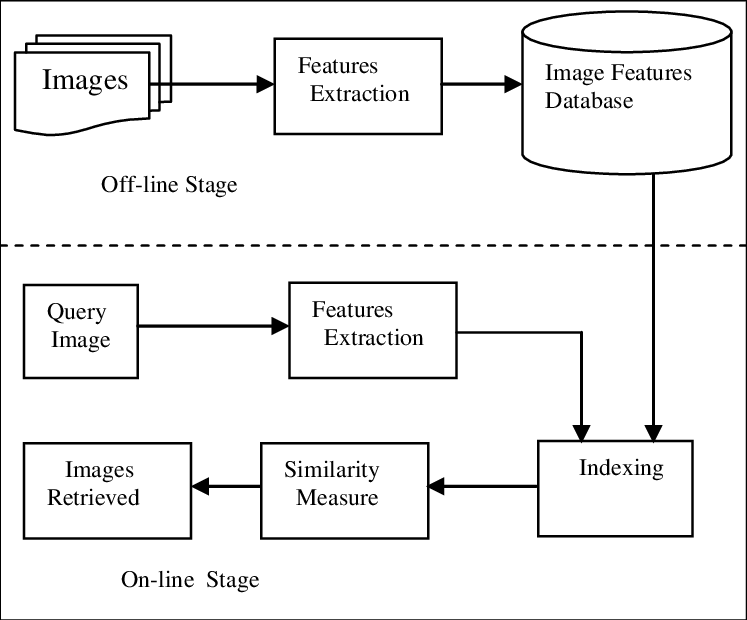
\includegraphics[width=1.0\textwidth]{images/image_retrieval_pipeline.png}
    \captionof{figure}{Sơ đồ hệ thống truy xuất ảnh dựa trên nội dung. Cơ sở dữ liệu ảnh được tiền xử lý và lập chỉ mục. Ảnh truy vấn được chuyển thành vector đặc trưng và so sánh với chỉ mục để tìm kết quả.}
    \label{fig:image_retrieval_pipeline}
\end{center}
\subsubsection{Phân loại/Nhận dạng Ảnh (Image Classification/Recognition)}
\label{subsubsec:image_classification}
\textbf{Bài toán:} Gán một ảnh vào một trong các lớp đã được định nghĩa trước (ví dụ: "chó", "mèo", "ô tô").

\textbf{Quy trình làm việc:}
\begin{enumerate}
    \item \textbf{Giai đoạn Huấn luyện (Training):}
    \begin{itemize}
        \item Giống như CBIR, bước đầu tiên là học một từ điển thị giác từ tập dữ liệu huấn luyện.
        \item Đối với mỗi ảnh trong tập huấn luyện, tính toán vector biểu diễn toàn cục (BoVW, VLAD, hoặc FV).
        \item Các vector này, cùng với nhãn lớp tương ứng của chúng, được sử dụng để huấn luyện một bộ phân loại (classifier). Do các vector này có chiều cao và thường có thể phân tách tuyến tính sau các bước chuẩn hóa, \textbf{Support Vector Machine (SVM) với kernel tuyến tính} là lựa chọn phổ biến và cực kỳ hiệu quả. Việc sử dụng kernel tuyến tính cho phép huấn luyện và dự đoán rất nhanh, ngay cả với số lượng lớp và mẫu lớn.
    \end{itemize}
    \item \textbf{Giai đoạn Dự đoán (Prediction):}
    \begin{itemize}
        \item Khi có một ảnh mới cần phân loại, hệ thống tính toán vector biểu diễn toàn cục của nó bằng cùng một từ điển.
        \item Vector này sau đó được đưa vào bộ phân loại SVM đã được huấn luyện để dự đoán nhãn lớp cho ảnh.
    \end{itemize}
\end{enumerate}
Pipeline "trích xuất đặc trưng -> mã hóa (FV/VLAD) -> SVM tuyến tính" đã là kiến trúc tiêu chuẩn và đạt hiệu năng state-of-the-art trên nhiều bộ dữ liệu phân loại ảnh kinh điển (như PASCAL VOC, Caltech-256) trong nhiều năm, cho đến trước khi bị các mạng nơ-ron tích chập sâu vượt qua vào khoảng năm 2012-2014. Tuy nhiên, các nguyên lý của nó vẫn là nền tảng quan trọng để hiểu về học biểu diễn trong thị giác máy tính.

\section*{Tài liệu tham khảo}
\begin{itemize}
    \item[1] Sánchez, J., Perronnin, F., Mensink, T., \& Verbeek, J. (2013). Image Classification with the Fisher Vector: Theory and Practice. \textit{International Journal of Computer Vision}, \textit{105}(3), 222–245.
    \item[2] Perronnin, F., \& Dance, C. (2007). Fisher kernels on visual vocabularies for image categorization. In \textit{2007 IEEE Conference on Computer Vision and Pattern Recognition (CVPR)}.
    \item[3] Jégou, H., Douze, M., Schmid, C., \& Pérez, P. (2010). Aggregating local descriptors into a compact image representation. In \textit{2010 IEEE Computer Society Conference on Computer Vision and Pattern Recognition (CVPR)}.
    \item[4] Jégou, H., Perronnin, F., Douze, M., Sánchez, J., Pérez, P., \& Schmid, C. (2012). Aggregating local image descriptors into compact codes. \textit{IEEE Transactions on Pattern Analysis and Machine Intelligence}, \textit{34}(9), 1704–1716.
    \item[5] Arandjelović, R., \& Zisserman, A. (2013). All about VLAD. In \textit{2013 IEEE Conference on Computer Vision and Pattern Recognition (CVPR)}.
    \item[6] Sivic, J., \& Zisserman, A. (2003). Video Google: A text retrieval approach to object matching in videos. In \textit{Proceedings of the Ninth IEEE International Conference on Computer Vision}.
    \item[7] Jaakkola, T. S., \& Haussler, D. (1999). Exploiting generative models in discriminative classifiers. In \textit{Advances in Neural Information Processing Systems 11 (NIPS 1998)}.
    \item[8] Gidaris, S., Bursuc, A., Komodakis, N., Pérez, P., \& Cord, M. (2020). Learning Representations by Predicting Bags of Visual Words. \textit{arXiv preprint arXiv:2002.12247}.
    \item[9] Lazebnik, S., Schmid, C., \& Ponce, J. (2006). Beyond bags of features: Spatial pyramid matching for recognizing natural scene categories. In \textit{2006 IEEE Computer Society Conference on Computer Vision and Pattern Recognition (CVPR'06)}.
    \item[10] Jégou, H., Douze, M., \& Schmid, C. (2011). Product quantization for nearest neighbor search. \textit{IEEE Transactions on Pattern Analysis and Machine Intelligence}, \textit{33}(1), 117–128.
    \item[11] Perronnin, F., Sánchez, J., \& Mensink, T. (2010). Improving the Fisher Kernel for large-scale image classification. In \textit{European Conference on Computer Vision (ECCV)}.
\end{itemize}
